\documentclass[../Master.tex]{subfiles}
\begin{document}

\begin{figure}
    \centering
    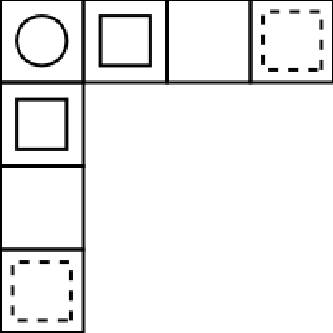
\includegraphics[scale=0.7]{Graphics/soko1}
    \caption{\label{fig:simpleSokoban} <\texttt{TODO:} redraw, one tile too many, label tiles> A simple sokoban world. The circle is the sokoban, the squares are crates, and the dashed lines denote goal tiles.}
\end{figure}

We will now present a formalization of the sokoban world introduced in section \ref{sec:Algorithm} based on the PDDL specification presented in \cite{BS2011}.

\subsubsection{Problem specification}
Any given sokoban problem, such as the one illustrated in figure \ref{fig:simpleSokoban}, contains a number of $crate$ objects (denoted $c_1, \dots, c_n$) as well as a number of $tile$ objects (denoted $t_1, \dots, t_k$). To describe how the tiles are interconnected, we introduce the predicates $hAdj(t_1,t_2)$ and $vAdj(t_1,t_3)$, respectively denoting that tile $t_1$ is horizontally adjacent to tile $t_2$ and vertically adjacent to $t_3$. It is clear that these relations are symmetric; if $t_i$ is vertically adjacent to $t_j$, then $t_j$ is also vertically adjacent to $t_i$ (similarly for horizontal adjacency). In the framework presented above, there is no machinery for aximoatic reasoning, hence this symmetry must be manually encoded by the problem designer by --- in the above example --- adding the predicates $hAdj(t_2,t_1)$ and $vAdj(t_3,t_1)$.

Locations of the crates can be encoded with the predicate $at(c, t)$, denoting that crate $c$ is on tile $t$. Locations of goal tiles and the sokoban are represented with the predicates $goal(t)$ and $sokobanAt(t)$, respectively.

The initial state of a problem can now be represented by a conjunction of the these predicates. The state illustrated in figure \ref{fig:simpleSokoban} can be encoded by the formula in \eqref{eq:simpleSokoSpec}. The \textit{goal} of any sokoban problem is that each crate is positioned at a goal tile, denoted by the conjunction $atGoal(c_1) \land atGoal(c_2) \land \cdots \land atGoal(c_n)$.

\begin{gather}
\begin{gathered} \label{eq:simpleSokoSpec}
    hAdj(t_1, t_2) \land hAdj(t_2, t_3) \land hAdj(t_3, t_4) \land \\
    hAdj(t_2, t_1) \land hAdj(t_3, t_2) \land hAdj(t_4, t_3) \land \\
    vAdj(t_1, t_5) \land vAdj(t_5, t_6) \land \\
    vAdj(t_5, t_1) \land vAdj(t_6, t_5) \land \\
    goal(t_4) \land goal(t_6) \land \\
    sokobanAt(t_1) \land at(c_1, t_2) \land at(c_2, t_5) \land \\
    clear(t_3) \land clear(t_4) \land clear(t_6)
\end{gathered}
\end{gather}

\end{document}
